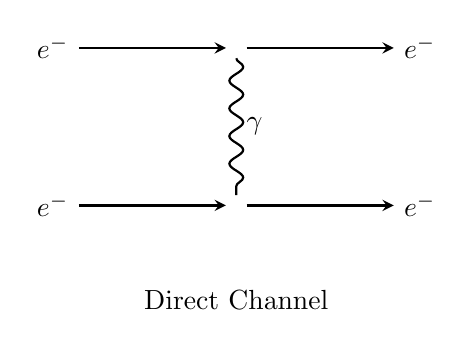
\begin{tikzpicture}[>=stealth, thick]

%--- Direct Channel ---
% Fermions in ingresso
\node[left] (a1) at (-2,1) {$e^-$};
\node[left] (a2) at (-2,-1) {$e^-$};

% Fermions in uscita
\node[right] (b1) at (2,1) {$e^-$};
\node[right] (b2) at (2,-1) {$e^-$};

% Vertici
\node (v1) at (0,1) {};
\node (v2) at (0,-1) {};

% Linee fermioniche
\draw[->] (a1) -- (v1);
\draw[->] (a2) -- (v2);
\draw[->] (v1) -- (b1);
\draw[->] (v2) -- (b2);

% Fotone
\draw[decorate, decoration={snake}] (v1) -- node[right] {$\gamma$} (v2);

% Titolo
\node at (0,-2.2) {Direct Channel};

\end{tikzpicture}
\hspace{2cm}
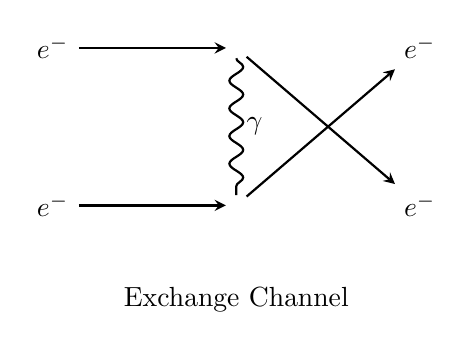
\begin{tikzpicture}[>=stealth, thick]

%--- Exchange Channel ---
% Fermions in ingresso
\node[left] (c1) at (-2,1) {$e^-$};
\node[left] (c2) at (-2,-1) {$e^-$};

% Fermions in uscita
\node[right] (d1) at (2,1) {$e^-$};
\node[right] (d2) at (2,-1) {$e^-$};

% Vertici
\node (v3) at (0,1) {};
\node (v4) at (0,-1) {};

% Linee fermioniche con scambio
\draw[->] (c1) -- (v3);
\draw[->] (c2) -- (v4);
\draw[->] (v3) -- (d2);
\draw[->] (v4) -- (d1);

% Fotone
\draw[decorate, decoration={snake}] (v3) -- node[right] {$\gamma$} (v4);

% Titolo
\node at (0,-2.2) {Exchange Channel};

\end{tikzpicture}
